\documentclass[]{scrartcl}

%opening
\title{Rotating magneto-hydrodynamics}
\author{J. Lara \& S. Glane}

\usepackage{amsmath}
\usepackage{amssymb}
\usepackage{amsfonts}
\usepackage{mathtools}
\usepackage{xfrac}
\usepackage{siunitx}
\usepackage{hyperref}
\usepackage{cleveref}
\usepackage{upgreek}
\newcommand{\pfrac}[2]{\frac{\partial #1}{\partial #2}}
\newcommand{\tdfrac}[2]{\frac{\mathrm{d} #1}{\mathrm{d} #2}}
\renewcommand{\d}{\,\mathrm{d}}
\newcommand{\bs}[1]{\boldsymbol{#1}}
\newcommand{\abs}[1]{\left\lvert #1 \right\rvert}
\newcommand{\norm}[1]{\left\lVert #1 \right\rVert}
\newcommand{\cdott}{\, {\cdot}{\cdot}\,}
\DeclareMathOperator{\divv}{div}
\DeclareMathOperator{\grad}{grad}
\DeclareMathOperator{\rot}{rot}
\DeclareMathOperator{\cof}{Cof}
\DeclareMathOperator{\Spur}{tr}
\DeclareMathOperator{\Sgn}{sgn}
\DeclareMathOperator{\Sym}{sym}

\newcommand{\alignedintertext}[1]{%
	\noalign{%
		\vskip\belowdisplayshortskip
		\vtop{\hsize=\linewidth#1\par
			\expandafter}%
		\expandafter\prevdepth\the\prevdepth
	}%
}

\begin{document}

\maketitle

\begin{abstract}

\end{abstract}

\section{Fluid mechanics}\label{Sec:FluidMechanics}
A \textbf{purely mechanical analysis} of a fluid reduces to the momentum and mass conservation. Their local forms are given by
\begin{subequations}\label{Eqn:FieldEqutaions}
	\begin{align}
		\label{Eqn:LinearMomemntum}
		\rho \tdfrac{\bs{v}}{t} &= \nabla \cdot \bs{T} + \rho \bs{b}, &\forall (\bs{x}, t) \in \Omega \times \left[0, T \right] \\
		\label{Eqn:MassConservation}
		\tdfrac{\rho}{t} + \rho \nabla \cdot \bs{v}&= 0, &\forall (\bs{x}, t) \in \Omega \times  \left[0, T \right]
	\end{align}
\end{subequations} 
where $\rho$ is the density, $\bs{v}$ the velocity, $\bs{T}$ the stress tensor and $\bs{b}$ the volumetric forces. Furthermore, $\bs{x}$ denotes the position vector, $t$ the time, $\Omega$  $n$-dimensional domain $\Omega \subset \mathbb{R}^n$ and $T$ the upper limit of the temporal space. The field equations need to be complemented with initial and boundary conditions and a constitutive equation for the stress in order for them to be solvable. For \textbf{linear viscous and isotropic} fluids the stress tensor is given by the \textsc{Navier-Stokes} law
\begin{equation*}
	\bs{T} = (-p + \lambda \Spur \bs{D}) \bs{I} + 2 \mu \bs{D}
\end{equation*}
Here, $p$ denotes the hydrostatic pressure, $\lambda$ the bulk viscosity, $\mu$ the dynamic viscosity, $\bs{D} = \Sym (\nabla \otimes \bs{v})$ the symmetric part of the velocity gradient and $\bs{I}$ the second order identity tensor. \textbf{Assuming that $\lambda$ and $\mu$ are constants}, the momentum field equation becomes
\begin{equation*}
\rho \tdfrac{\bs{v}}{t} = -\nabla p + (\lambda + \mu) \nabla (\nabla \cdot \bs{v}) + \mu \Delta \bs{v} + \rho\bs{b}, \quad \forall (\bs{x}, t) \in \Omega \times \left[0, T \right]
\end{equation*}
For the case of an \textbf{incompressible fluid}, i.e. $\nabla \cdot \bs{v} = 0$, and expanding the material time derivative, the field equations reduce further to
\begin{equation*}
	\begin{aligned}
		\rho \pfrac{\bs{v}}{t} +  \rho \bs{v} \cdot (\nabla \otimes \bs{v})&=  -\nabla p + \mu \Delta \bs{v} + \rho \bs{b}, &\forall (\bs{x}, t) \in \Omega \times \left[0, T \right] \\
		\nabla \cdot \bs{v}&= 0, &\forall (\bs{x}, t) \in \Omega \times  \left[0, T \right]
	\end{aligned}
\end{equation*}
\textbf{Assuming that density is constant}, it is customary to divide the momentum equation by it, which yields to 
\begin{subequations}\label{Eqn:ReducedFieldEquations}
	\begin{align}
		\label{Eqn:ReducedNavierStokesLinearMommentum}
		\pfrac{\bs{v}}{t} + \bs{v} \cdot (\nabla \otimes \bs{v})&=  - \dfrac{1}{\rho}\nabla p + \nu \Delta \bs{v} + \bs{b}, &\forall (\bs{x}, t) \in \Omega \times \left[0, T \right] \\
		\label{Eqn:ReducedNavierStokesMassConservation}
		\nabla \cdot \bs{v}&= 0, &\forall (\bs{x}, t) \in \Omega \times  \left[0, T \right]
	\end{align}
\end{subequations}
where $\nu = \sfrac{\mu}{\rho}$ is the kinematic viscosity. The dimensionless form of this set of field equations is obtained by introducing a multiplicative decomposition of an arbitrary tensor $\bs{\phi}$
\begin{equation*}
	\bs{\phi} = \hat{\phi} \tilde{\bs{\phi}}
\end{equation*}
Here, $\hat{\phi}$ is a constant dimensional scalar, which is regarded as an scaling factor, and $ \tilde{\bs{\phi}}$ is a dimensionless tensor. By implementing the decomposition, the field equations become
\begin{subequations}\label{Eqn:AdimensionalReducedFieldEquations}
	\begin{align}
		\label{Eqn:DimensionlessReducedNavierStokesLinearMommentum}
		\pfrac{\bs{\tilde{v}}}{\tilde{t}} + \bs{\tilde{v}} \cdot (\tilde{\nabla} \otimes \bs{\tilde{v}})&=  -\tilde{\nabla} \tilde{p}+ \dfrac{1}{\mathrm{Re}}\tilde{\Delta} \bs{\tilde{v}} + \bs{\tilde{b}}, &\forall (\bs{\tilde{x}}, \tilde{t}) \in \tilde{\Omega} \times [0, \tilde{T} ] \\
		\label{Eqn:DimensionlessReducedNavierStokesMassConservation}
		\tilde{\nabla} \cdot \bs{\tilde{v}}&= 0, &\forall (\bs{\tilde{x}}, \tilde{t}) \in\tilde{ \Omega} \times  [0, \tilde{T} ]
	\end{align}
\end{subequations}
where $\mathrm{Re} = \hat{v}L_\textrm{c}\nu^{-1}$ is the \textsc{Reynolds} number. Note that the scaling factor of the position vector is set as a characteristic length of the problem, i.e. $\hat{x} = L_\textrm{c}$. Consistently, the characteristic time is set to $\hat{t} = \sfrac{L_\textrm{c}}{\hat{v}}$. Furthermore, pressure scaling and volumemetric force scaling were set to $\hat{p} = \rho \hat{v}^2$ and $\hat{b} = \hat{v}\hat{t}^{-1}$ respectively. \textbf{From here on now the tildes are going to be obviated, but keep in mind we are working with the dimensionless form of the field equations}.\\

\section{Treatment of the convection term}
The convective term $\bs{v} \cdot (\nabla \otimes \bs{v})$ might be replaced by another expression, which would reduce back to  $\bs{v} \cdot (\nabla \otimes \bs{v})$ or are rendered equivalent to it  by imposing the divergence free condition. Among these form are
\begin{itemize}
	\item the skew-symmetric form
	\begin{equation}
		\label{Eqn:SkewSymmetricForm}
		\frac{1}{2}\bs{v} \cdot (\nabla \otimes \bs{v}) + \dfrac{1}{2} 	\nabla \left( \bs{v} \otimes \bs{v}\right) = \bs{v} \cdot (\nabla \otimes \bs{v}) + \dfrac{1}{2}(\nabla \cdot \bs{v})\bs{v}
	\end{equation}
	\item the divergence form
	\begin{equation}
		\label{Eqn:DivergenceForm}
		\nabla \left( \bs{v} \otimes \bs{v}\right) = \bs{v} \cdot (\nabla \otimes \bs{v}) + (\nabla \cdot \bs{v})\bs{v}
	\end{equation}
	\item and the rotational form
	\begin{equation}
		\label{Eqn:RotationalForm}
		\bs{v} \cdot (\nabla \otimes \bs{v}) = (\nabla \times \bs{v}) \times \bs{v} + \dfrac{1}{2} \nabla \norm{\bs{v}}^2
	\end{equation}
	where is customary to define the dynamic, or total, pressure $P = p +  \tfrac{1}{2} \norm{v}^2$ and solve the problem for $P$ instead.
\end{itemize}


\section{Projection methods: Pressure-correction schemes}
The momentum equation and mass conservation field equations are meant to be solved simultaneously to find $\bs{v}$ and $p$. For large problems this can be cumbersome and slow, since a proper preconditioner requires more work and the system to solve is bigger. The projection methods aim to decouple the field equations. In the case of the pressure-correction schemes this is done by introducing an auxiliary velocity field $\bs{u}$, which is not divergence free, and splitting the momentum equation into two equations. This is better explained by looking specific schemes up. We formally define the problem
\begin{alignat*}{2}
	\pfrac{\bs{v}}{t}  + \bs{v}\cdot (\nabla \otimes \bs{v}) &=  -\nabla p  +  \mathrm{Re}^{-1} \Delta \bs{v} + \bs{b}, \quad &\forall (\bs{x}, t) &\in \Omega \times \left[0, T \right] \\
	\nabla \cdot \bs{v} &= 0, &\forall (\bs{x}, t) &\in \Omega \times \left[0, T \right] \\
	\intertext{with boundary conditions,}
	\bs{v} &= \bs{v}_\textrm{D} &\forall\left(\bs{x}, t\right) &\in \Gamma_\textrm{D} \times \left[0, T \right] \\ 
	[-p \bs{I} + \textrm{Re}^{-1}\nabla \otimes \bs{v}]\cdot \bs{n} &= \bs{t}_\textrm{N}, &\forall \left(\bs{x}, t\right) &\in \Gamma_\textrm{N} \times \left[0, T \right] \\
	\intertext{and initial condtion,} 
	\bs{v} &= \bs{v}_0, &\forall (\bs{x}, 0) &\in \Omega
\end{alignat*}
where $\bs{v}_\textrm{D}$ denotes the velocity at the \textsc{Dirichlet} boundary $\Gamma_\textrm{D}\subset\partial\Omega$, $\bs{t}_\textrm{N}$ the traction vector at the \textsc{Neumann} boundary $\Gamma_\textrm{N}\subset\partial\Omega$, $\bs{t}_\textrm{N}$, with $\partial \Omega = \Gamma_\textrm{D} \cup \Gamma_\textrm{N}$ and $ \Gamma_\textrm{D} \cap \Gamma_\textrm{N} = \emptyset$, and $\bs{v}_0$ is the initial velocity. As a remainder, the stated problem is dimensionless. Therefore the boundary and initial conditions are also expressed in their dimensionless form.
\subsection{Incremental scheme in standard form}
By implementing a BDF2 scheme for the time derivative and adding and subtracting an auxiliary velocity field $\bs{u}$, which is not divergence free but fulfills the \textsc{Dirichlet} boundary conditions, and the pressure from the previous time step to the mix we obtain
\begin{equation*}
\begin{split}
	\dfrac{1}{2\Delta t} \left[3\bs{v}^{k} + 3\bs{u}^{k} - 3\bs{u}^{k} - 4\bs{v}^{k-1} + \bs{v}^{k-2}\right]  + \bs{v}^{k} \cdot (\nabla \otimes \bs{v}^{k})= \\  -\nabla (p^{k} + p^{k-1} - p^{k+1}) +  \mathrm{Re}^{-1} \Delta \bs{v}^{k} + \bs{b}^{k}
\end{split}
\end{equation*}
which is now split into
\begin{subequations}
	\begin{align}
		\label{Eqn:PreDiffusionEquation}
		\dfrac{1}{2\Delta t} \left[3\bs{u}^{k} - 4\bs{v}^{k-1} + \bs{v}^{k-2}\right]  + \bs{v}^{k} \cdot (\nabla \otimes \bs{v}^{k}) &= -\nabla p^{k-1} +  \mathrm{Re}^{-1} \Delta \bs{v}^{k} + \bs{b}^{k} 
		\\
		\label{Eqn:PreProjectionEquation}
		\dfrac{0.5}{\Delta t} \left[3\bs{v}^{k} - 3\bs{u}^{k} \right] &= -\nabla (p^{k} - p^{k-1})
	\end{align}
\end{subequations}
The decoupling takes places by replacing $\bs{v}^{k}$ by $\bs{u}^{k}$ in the convective and diffusive terms and solving \cref{Eqn:PreDiffusionEquation} without taking the incompressibilty condition in consideration, i.e.
\begin{equation*}
	\begin{aligned}
		\dfrac{0.5}{\Delta t} \left[3\bs{u}^{k} - 4\bs{v}^{k-1} + \bs{v}^{k-2}\right]  + \bs{u}^{k} \cdot (\nabla \otimes \bs{u}^{k}) &= -\nabla p^{k-1} +  \mathrm{Re}^{-1} \Delta \bs{u}^{k} + \bs{b}^{k}, &\forall (\bs{x}, t) &\in \Omega \times \left[0, T \right]  \\
		\bs{u}^{k} &= \bs{v}_\textrm{D}, &\forall (\bs{x}, t) &\in \Gamma_\textrm{D} \times \left[0, T \right] \\
		[-p^{k-1} \bs{I} + (\textrm{Re})^{-1}\nabla \otimes \bs{u}^{k}]\cdot \bs{n} &= \bs{t}_\textrm{N}, &\forall \left(\bs{x}, t\right) &\in \Gamma_\textrm{N} \times \left[0, T \right]
	\end{aligned}
\end{equation*}
which is called the viscous or diffusion step. The \cref{Eqn:PreProjectionEquation} is coupled with the incompressibility condition to form the projection step
\begin{equation*}
\begin{aligned}
		\dfrac{1}{2\Delta t} \left[3\bs{v}^{k} - 3\bs{u}^{k} \right] &= -\nabla (p^{k} - p^{k-1}), &\forall (\bs{x}, t) &\in \Omega \times \left[0, T \right] \\
		\nabla \cdot \bs{v}^{k} &= 0, &\forall (\bs{x}, t) &\in \Omega \times \left[0, T \right] \\
	\nabla(p^{k} - p^{k-1}) \cdot \bs{n} &= 0, &\forall (\bs{x}, t) &\in \Gamma_\textrm{D} \times \left[0, T \right] \\
		p^{k} - p^{k-1} &=0, &\forall\left(\bs{x}, t\right) &\in \Gamma_\textrm{N} \times \left[0, T \right]
\end{aligned}	
\end{equation*}
By applying the divergence operator to the equation and introducing an auxiliary variable $\phi^{k} = p^{k} - p^{k-1}$ , the whole step can be reduced to
\begin{equation*}
\begin{aligned}
	\Delta \phi^{k} &= \dfrac{1.5}{\Delta t} \nabla \cdot \bs{u}^{k},  &\forall (\bs{x}, t) &\in \Omega \times \left[0, T \right] \\
	\nabla \phi^{k} \cdot \bs{n} &= 0, &\forall (\bs{x}, t) &\in \Gamma_\textrm{D} \times \left[0, T \right] \\
	\phi^{k} &= 0, &\forall\left(\bs{x}, t\right) &\in \Gamma_\textrm{N} \times \left[0, T \right]
\end{aligned}
\end{equation*}
The first boundary condition is an artificial boundary condition which reduces the order of the scheme in its $L^2$ and $H^1$ norms. The last step of the pressure-correction scheme is called correction or update step. As the name implies the velocity $\bs{v}^{k}$ and pressure $p^{k}$ are computed by
\begin{equation*}
\begin{aligned}
	\bs{v}^{k} &= \bs{u}^{k} - \dfrac{2\Delta t}{3} \nabla \phi^{k} \\
	p^{k} &= p^{k-1} + \phi^{k}
\end{aligned}
\end{equation*}
\subsection{Incremental scheme in rotational form}
The rotational form implements the same diffusion step
\begin{equation*}
	\begin{aligned}
		\dfrac{1}{2\Delta t} \left[3\bs{u}^{k} - 4\bs{v}^{k-1} + \bs{v}^{k-2}\right]  + \bs{u}^{k} \cdot (\nabla \otimes \bs{u}^{k}) &= -\nabla p^{k-1} +  \mathrm{Re}^{-1} \Delta \bs{u}^{k} + \bs{b}^{k}, &\forall (\bs{x}, t) &\in \Omega \times \left[0, T \right]  \\
		\bs{u}^{k} &= \bs{v}_\textrm{D}, &\forall (\bs{x}, t) &\in \Gamma_\textrm{D} \times \left[0, T \right] \\
		[-p^{k-1} \bs{I} + (\textrm{Re})^{-1}\nabla \otimes \bs{u}^{k}]\cdot \bs{n} &= \bs{t}_\textrm{N}, &\forall \left(\bs{x}, t\right) &\in \Gamma_\textrm{N} \times \left[0, T \right]
	\end{aligned}
\end{equation*}
and the same scheme of projection step
\begin{equation*}
	\begin{aligned}
		\Delta \phi^{k} &= \dfrac{2}{3\Delta t} \nabla \cdot \bs{u}^{k},  &\forall (\bs{x}, t) &\in \Omega \times \left[0, T \right] \\
		\nabla \phi^{k} \cdot \bs{n} &= 0, &\forall (\bs{x}, t) &\in \Gamma_\textrm{D} \times \left[0, T \right] \\
		\phi^{k} &= 0, &\forall\left(\bs{x}, t\right) &\in \Gamma_\textrm{N} \times \left[0, T \right]
	\end{aligned}
\end{equation*}
with the exception that the auxiliary variable is defines as
\begin{equation*}
	\phi^{k} = p^{k} - p^{k-1} + \textrm{Re}^{-1} \nabla \cdot \bs{u}^{k}
\end{equation*}
The update of the velocity and the pressure is given then by
\begin{equation*}
	\begin{aligned}
		\bs{v}^{k} &= \bs{u}^{k} - \dfrac{2\Delta t}{3} \nabla \phi^{k} \\
		p^{k} &= p^{k-1} + \phi^{k} -  \textrm{Re}^{-1} \nabla \cdot \bs{u}^{k}
	\end{aligned}
\end{equation*}
 From the first equation of the projection step, before applying the divergence to it, 
\begin{equation*}
\dfrac{1}{2\Delta t} \left[3\bs{v}^{k} - 3\bs{u}^{k} \right] = -\nabla \phi^{k}
\end{equation*}
it is easy to see that $\nabla \times \nabla \times \bs{u}^k = \nabla \times \nabla \times \bs{v}^k$. Furthermore by adding the above equation to the diffusion step, using the identity $\nabla \times \nabla \times \bs{a} = \nabla (\nabla \cdot \bs{a}) - \Delta \bs{a}$ and coupling the result again with the incompressibility condition we get the \textsc{Navier-Stokes} equations again. This form greatly improves the deficiencies of the standard form due to boundary layer created by the artifical boundary condition. 

\subsection{Generalized incremental scheme}
The standard and rotational forms can be generalized into one scheme using a backward difference formula of $q$-order (BDF$q$) by defining the time derivative
\begin{equation*}
	\pfrac{\bs{v}}{t} = \dfrac{1}{\Delta t}\left[ \zeta_q \bs{u}^{k} - \sum_{j=1}^{q} \zeta_j \bs{v}^{k-j}\right]
\end{equation*}
and the $r$-th order extrapolation of the pressure 
\begin{equation*}
	p^{\star, k} = \sum_{j=1}^{r} \eta_j p^{k-j}
\end{equation*}
The diffusion step is then given by
\begin{equation*}
	\begin{aligned}
		\dfrac{1}{\Delta t} \left[\zeta_q \bs{u}^{k} - \sum_{j=1}^{q} \zeta_j \bs{v}^{k-j}\right]  + \bs{u}^{k} \cdot (\nabla \otimes \bs{u}^{k}) &= -\nabla	p^{\star, k} +  \mathrm{Re}^{-1} \Delta \bs{u}^{k} + \bs{b}^{k}, &\forall (\bs{x}, t) &\in \Omega \times \left[0, T \right]  \\
		\bs{u}^{k} &= \bs{v}_\textrm{D}, &\forall (\bs{x}, t) &\in \Gamma_\textrm{D} \times \left[0, T \right] \\
		[-	p^{\star, k} \bs{I} + (\textrm{Re})^{-1}\nabla \otimes \bs{u}^{k}]\cdot \bs{n} &= \bs{t}_\textrm{N}, &\forall \left(\bs{x}, t\right) &\in \Gamma_\textrm{N} \times \left[0, T \right]
	\end{aligned}
\end{equation*}
and the projection step by
\begin{equation*}
	\begin{aligned}
		\Delta \phi^{k} &= \dfrac{\zeta_q}{\Delta t} \nabla \cdot \bs{u}^{k},  &\forall (\bs{x}, t) &\in \Omega \times \left[0, T \right] \\
		\nabla \phi^{k} \cdot \bs{n} &= 0, &\forall (\bs{x}, t) &\in \Gamma_\textrm{D} \times \left[0, T \right] \\
		\phi^{k} &= 0, &\forall\left(\bs{x}, t\right) &\in \Gamma_\textrm{N} \times \left[0, T \right]
	\end{aligned}
\end{equation*}
with an auxiliary variable defined as
\begin{equation*}
	\phi^{k} = p^{k} - p^{\star, k} + \chi\textrm{Re}^{-1} \nabla \cdot \bs{u}^{k}
\end{equation*}
where the parameter $\chi$ is set to 0 and 1 for the standard and rotational form respectively. The update step follows as usual.
\subsubsection{Elimination of the divergence free velocity}
The velocity field $\bs{v}$ is indeed divergence free but it does not satisfy the boundary conditions, whilst the velocity field $\bs{u}$ has the opposite qualities. From an accuracy point of view they are equivalent since they yield the same error estimates. One may choose to eliminate the velocity field $\bs{v}$ by noting that the \textsc{Poisson} equation of the projection step holds naturally for all previous $\bs{v}^{k-j}$ and $\bs{u}^{k-j}$ $\forall j\ge 1$. Multiplying it by $\zeta_j$ leads to
\begin{equation*}
	\dfrac{\zeta_j}{\Delta t} \left[\bs{v}^{k-j} - \bs{u}^{k-j} \right] = -\nabla \left(\dfrac{\zeta_j}{\zeta_q}\phi^{k-j}\right)
\end{equation*}
Solving for $\bs{v}^{k-j}$ and replacing it in the diffusion step leads to
\begin{equation*}
		\dfrac{1}{\Delta t} \left[\zeta_q \bs{u}^{k} - \sum_{j=1}^{q} \zeta_j \bs{u}^{k-j}\right]  + \bs{u}^{k} \cdot (\nabla \otimes \bs{u}^{k}) = -\nabla	\left[p^{\star, k} + \sum_{j=1}^{q} \dfrac{\zeta_j}{\zeta_q}\phi^{k-j} \right] +  \mathrm{Re}^{-1} \Delta \bs{u}^{k} + \bs{b}^{k}.
\end{equation*}
while the rest of the equations remain the same.
\section{Implementation of the variable step size implicit-explicit linear multistep time discretization schemes to the pressure-correction methods}
Until now we have been implementing a BDF2 scheme to the time derivative, but the projection method is not limited to it, other consistent schemes are also admissible. With this in mind, we take the generalized incremental scheme after that elimination of the divergence free velocity and implement the variable step size implicit-explicit linear multistep time discretization scheme (VSIMEX). Considering the equation
\begin{equation*}
	\pfrac{u}{t} = f(u, t) + g(u, t) + h(u, t)
\end{equation*}
where $f(u, t)$ is a nonstiff and possibly nonlinear term, which will be integrated explicitly, $g(u,  t)$ a stiff term, which will be integrated implicitly and $h(u, t)$ a term whose treatment is independent from the VSIMEX scheme. This last term is a small modification of the VSIMEX scheme proposed by the authors. All the term may also be dependent of other variables. The general form of the $s$-th order VSIMEX scheme is given by
\begin{equation*}
	\dfrac{1}{\Delta t_{k-1}} \sum_{j=0}^{s} \alpha_i^k u^{k-j} = \sum_{j=1}^{s} \beta_i^k f(u^{k-j}, t^{k-j}) + \sum_{j=0}^{s} \gamma_i^k g(u^{k-j}, t^{k-j})
\end{equation*}
The coefficients $\alpha^k$, $\beta^k$ and $\gamma^k$ are defined by different input parameters depending on the order of the scheme and the previous time step. We wish now to implement the above general form to our generalized incremental scheme. First, let us define
\begin{equation*}
	\begin{aligned}
		f(\bs{u}, \dots) &= -\bs{u} \cdot (\cdot \otimes \bs{u}) + \bs{b}(\dots) \\
		g(\bs{u}) &= \textrm{Re}^{-1} \Delta \bs{u} \\
		h(p, \phi)	 &= -\nabla p^\sharp
	\end{aligned}
\end{equation*}
The treatment of $h(p,\phi)$ is dictated by the incremental pressure correction scheme, its definition will be explained shortly. Extracting the first term of the explicit summation leads to
\begin{equation*}
\dfrac{1}{\Delta t_{k-1}} \left[\alpha_0^k \bs{u}^{k} + \sum_{j=1}^{s} \alpha_i^k \bs{u}^{k-j}\right] - \gamma_0^k g(\bs{u}^{k}) = \sum_{j=1}^{s} \beta_i^k f(\bs{u}^{k-j},\dots) + \sum_{j=1}^{s} \eta_i^k g(\bs{u}^{k-j}) + h(\phi)
\end{equation*}
Noticing that the first term of the equation mirrors, up to a sign, the algebraic form used to eliminate the divergence free velocity of the generalized incremental scheme and the above definitions of $f$ and $g$, we propose $s$th-order scheme with a \textbf{diffusion step}
\begin{equation}
\begin{split}\label{Eqn:VSIMEXDiffusionStep}
	\dfrac{\alpha_0^k}{\Delta t_{k-1}} \bs{u}^{k} -\dfrac{\gamma_0^k}{\textrm{Re}} \Delta \bs{u}^{k} = -\nabla p^{\sharp} + \sum_{j=1}^{s} \beta_i^k \left[ \bs{b} - \bs{u}^{k-j} \cdot (\nabla \otimes \bs{u}^{k-j})\right] + \\
	\sum_{j=1}^{s} \dfrac{\gamma_i^k}{\textrm{Re}} \Delta \bs{u}^{k-j} -   \sum_{j=1}^{s} \dfrac{\alpha_i^k}{\Delta t_{k-1}}\bs{u}^{k-j}, \qquad \forall(\bs{x},t)\in \Omega \times [0, T]
\end{split}
\end{equation}
with
\begin{equation*}
	 p^\sharp = p^{\star, k} - \sum_{j=1}^{s} \frac{\Delta t_{k-1-j}}{\Delta t_{k-1}}          \frac{\alpha_j^k}{\alpha_0^{k-j}}\phi^\textrm{k-j} ,
	 \qquad
	 p^{\star, k} = \sum_{j=1}^{r} \eta_j p^{k-j}
\end{equation*}
where $s\ge r$, with boundary conditions
\begin{equation*}
	\begin{aligned}
		\bs{u}^{k} &= \bs{v}_\textrm{D}, &\forall(\bs{x}, t) &\in \Gamma_\textrm{D} \times [0, T] \\
		[- p^{\star, k} \bs{I} + \textrm{Re}^{-1} \Sym (\nabla \otimes \bs{u}^{k})] \cdot \bs{n} &= \bs{t}_\textrm{N},  &\forall(\bs{x}, t) &\in \Gamma_\textrm{N} \times [0, T]
	\end{aligned}
\end{equation*}
a \textbf{projection step}

\begin{align}
\Delta \phi^{k} &= \dfrac{\alpha_0^k}{\Delta t} \nabla \cdot \bs{u}^{k},  &\forall (\bs{x}, t) &\in \Omega \times \left[0, T \right] \label{Eqn:VSIMEXProjectionStep} \\
\nabla \phi^{k} \cdot \bs{n} &= 0, &\forall (\bs{x}, t) &\in \Gamma_\textrm{D} \times \left[0, T \right] \nonumber \\
\phi^{k} &= 0, &\forall\left(\bs{x}, t\right) &\in \Gamma_\textrm{N} \times \left[0, T \right] \nonumber
\end{align}

and a \textbf{correction step}
\begin{equation}\label{Eqn:VSIMEXCorrectionStep}
	p^{k} = p^{\star, k} + \phi^{k} - \chi\textrm{Re}^{-1} \nabla \cdot \bs{u}^{k}
\end{equation}
\subsection{A semi-implicit approach}\label{Sec:SemiImplicit}
An alternative follows from introducing the $r$th-oder extrapolation of the velocity field $\bs{u}$ 
\begin{equation*}
\bs{u}^{\star, k} = \sum_{j=1}^{r} \eta_j \bs{u}^{k-j}
\end{equation*}
in order to linearize the convective term (in any of its forms) and treating it implicitly. That is to say, we define
\begin{equation*}
\begin{aligned}
f(\dots) &= \bs{b}(\dots) \\
g(\bs{u}) &= \textrm{Re}^{-1} \Delta \bs{u}\\
h(\bs{u}, \phi) &= -\nabla p^\sharp - \bs{u} \cdot (\nabla \otimes \bs{u})
\end{aligned}
\end{equation*}
and treat the convective term outside of the VSIMEX scheme, as we did with the pressure gradient. For example, the skew-symmetric form becomes
\begin{equation*}
	\bs{u}^{\star, k} \cdot (\nabla \otimes \bs{u}^{k}) + \dfrac{1}{2} (\nabla \cdot \bs{u}^{\star, k})\bs{u}^{k}
\end{equation*}

\subsection{The step-35 approach}\label{Sec:Step35}
The step-35 uses the generalized incremental scheme of second order (BDF2), the elimination of the divergence free velocity and a semi-implicit approach on the skew-symmetric form of the convective term, which leads to a projection step
\begin{equation*}
	\begin{split}
		\dfrac{1.5}{\Delta t} \bs{u}^{k} - \dfrac{1}{\textrm{Re}}\Delta \bs{u}^{k} + 	\bs{u}^{\star, k} \cdot (\nabla \otimes \bs{u}^{k}) + \dfrac{1}{2} (\nabla \cdot \bs{u}^{\star, k})\bs{u}^{k} = \hspace{5cm} \\ -\nabla p^\sharp - \left[-\dfrac{2}{\Delta t}\bs{u}^{k-1} + \dfrac{0.5}{\Delta t}\bs{u}^{k-2}\right] + \bs{b},  \qquad \forall(\bs{x},t)\in \Omega \times [0, T]
	\end{split}
\end{equation*}
where
\begin{equation*}
p^\sharp = p^{k-1} + \dfrac{4}{3} \phi^{k-1} - \dfrac{1}{3} \phi^{k-2}
\end{equation*}
with boundary condition
\begin{equation*}
\begin{aligned}
\bs{u}^{k} &= \bs{v}_\textrm{in},  &\forall(\bs{x}, t) &\in \Gamma_0 \times [0, T] \\
\bs{u}^{k} \times \bs{n}&= \bs{0}, &\forall(\bs{x}, t) &\in \Gamma_1 \times [0, T] \\
\bs{u}^{k} &= \bs{0}, &\forall(\bs{x}, t) &\in \Gamma_2 \times [0,T]\\
\bs{u}^{k} &= \bs{0}, &\forall(\bs{x}, t) &\in \Gamma_3 \times [0, T]
\end{aligned}
\end{equation*}
A correction step with
\begin{equation*}
\begin{aligned}
\Delta \phi^{k} &= \dfrac{1.5}{\Delta t} \nabla \cdot \bs{u}^{k},  &\forall (\bs{x}, t) &\in \Omega \times \left[0, T \right] \\
\nabla \phi^{k} \cdot \bs{n} &= 0, &\forall (\bs{x}, t) &\in \partial\Omega /\Gamma_\textrm{1} \times \left[0, T \right] \\
\phi^{k} &= 0, &\forall\left(\bs{x}, t\right) &\in \Gamma_1 \times \left[0, T \right]
\end{aligned}
\end{equation*}
and a correction step
\begin{equation*}
p^{k} = p^{k-1} + \phi^{k} - \chi\textrm{Re}^{-1} \nabla \cdot \bs{u}^{k}
\end{equation*}

\section{Numerical treatment}
The problem described in the \cref{Sec:FluidMechanics} will be solved using the finite element method, which is based upon the weak formulation of the problem and the proper selection and discretization of the trial and test function spaces.
\subsection{Weak formulation}
The weak formulation of diffusion and correction step is obtained by multiplying the \cref{Eqn:VSIMEXDiffusionStep,Eqn:VSIMEXProjectionStep} by the test functions $\bs{\nu}$ and $\omega$ respectively; applying the \textsc{Gauss} theorem where possible and assuming there are no \textsc{Neumann} boundary conditions; and applying a \textsc{Galerkin} space reduction the discrete problem becomes: Find $(\bs{u}^k_\textrm{h}, \phi^k_\textrm{h}) \in (V_{\bs{u}}, V_\phi)$ that fulfills
\begin{equation*}
\begin{split}
\dfrac{\alpha_0^k}{\Delta t^{k-1}} 
\int_{\Omega}
\bs{\nu} \cdot \bs{u}^k_\textrm{h}
\d v 
+ 
\dfrac{\gamma_0^k}{\textrm{Re}}
\int_{\Omega} 
\nabla \otimes \bs{\nu} \cdott \nabla \otimes \bs{u}^k_\textrm{h}
\d v
=
\int_{\Omega}
(\nabla \cdot \bs{\nu}) p^{\sharp, k}_\textrm{h}
\d v \\
-
\int_{\Omega}
\sum_{j=1}^{s} 
\left[
\dfrac{\alpha_j^k}{\Delta t^{k-1}} \bs{\nu} \cdot \bs{u}^{k-j}_\textrm{h}
+
\beta_j^k \bs{\nu} \cdot \left[ \bs{u}^{k-j}_\textrm{h} \cdot (\nabla \otimes \bs{u}^{k-j}_\textrm{h} ) - \bs{b} \right]
+
\dfrac{\gamma_j^k}{\textrm{Re}} \nabla \otimes \bs{\nu} \cdott \nabla \otimes \bs{u}^{k-j}_\textrm{h}
\right]
\d v
\end{split} 	
\end{equation*}
and 
\begin{equation*}
	\int_{\Omega}
	\nabla \omega \cdot \nabla \phi^k_\textrm{h} 
	\d v
	= 
	- \dfrac{\alpha_0^k}{\Delta t^{k-1}} 
	\int_{\Omega}
	\omega (\nabla \cdot \bs{u}^k_\textrm{h})
	\d v,
	\qquad
	\forall (\bs{\nu}, \omega) \in (W_{\bs{u}}, W_\phi)
\end{equation*}
where $(V_{\bs{u}}, V_\phi)$ and $(W_{\bs{u}}, W_\phi)$ are the discrete trial function spaces and the test functions spaces respectively. The linear equation systems are then given by
\begin{equation*}
	\left[
	\dfrac{\alpha_0^k}{\Delta t^{k-1}} 
	\mathcal{M}^u_{ij}
	+
	\dfrac{\gamma_0^k}{\textrm{Re}}
	\mathcal{K}^u_{ij}
	\right]
	U^k_J
	= 
	b^{u, k}_i
	\qquad \textrm{and} \qquad
	\mathcal{M}^\phi_{ij} \Phi^k_j = b^{\phi, k}_i
\end{equation*}
The matrices $\mathcal{M}_u$ and $\mathcal{M}_\phi$ are the mass matrices of the velocity and pressure respectively, whereas $\mathcal{K}_u$ is the stiffness matrix of the velocity, i.e.
\begin{equation*}
	\mathcal{M}^u_{ij}= \int_{\Omega} \bs{\psi}_i \cdot \bs{\psi}_j \d v,
	\qquad
	\mathcal{K}^u_{ij} = \int_{\Omega} \nabla \otimes \bs{\psi}_i \cdott \nabla \otimes \bs{\psi}_j \d v,
	\qquad \textrm{and} \qquad
	\mathcal{M}^\phi_{ij} = \int_{\Omega} \psi_i \psi_j \d v.
\end{equation*}
and the right hand sides are 
\begin{equation*}
\begin{split}
	b^u_i &= \int_{\Omega}
\Bigg\lbrace
(\nabla \cdot \bs{\psi}_i) p^{\sharp, k}_\textrm{h}
- \\
&\sum_{j=1}^{s} 
\left[
\dfrac{\alpha_j^k}{\Delta t^{k-1}} \bs{\psi}_i \cdot \bs{u}^{k-j}_\textrm{h}
+
\beta_j^k \bs{\psi}_i \cdot \left[ \bs{u}^{k-j}_\textrm{h} \cdot (\nabla \otimes \bs{u}^{k-j}_\textrm{h} ) - \bs{b} \right]
+
\dfrac{\gamma_j^k}{\textrm{Re}} \nabla \otimes \bs{\nu}_i \cdott \nabla \otimes \bs{u}^{k-j}_\textrm{h}
\right]\Bigg\rbrace
\d v
\end{split}
\end{equation*}
and
\begin{equation*}
\begin{aligned}
b^\phi_i  = 	- \dfrac{\alpha_0^k}{\Delta t^{k-1}} 
\int_{\Omega}
\omega_i (\nabla \cdot \bs{u}^k_\textrm{h})
\d v
\end{aligned}
\end{equation*}
This linear equation system is obtained by setting the \texttt{vsimex\_method\_flag} and \\ \texttt{semi\_implicit\_convection\_flag} to \texttt{true} and \texttt{false} respectively.
\subsubsection{A semi implicit approach}
The weak formulation of the equations described in \cref{Sec:SemiImplicit} leads to a linear equation system for the diffusion step
\begin{equation*}
	\left[
	\dfrac{\alpha_0^k}{\Delta t^{k-1}} 
	\mathcal{M}^u_{ij}
	+
	\dfrac{\gamma_0^k}{\textrm{Re}}
	\mathcal{K}^u_{ij}
	+
	\mathcal{C}^u_{ij}
	\right]
	U^k_J
	= 
	b^{u, k}_i
\end{equation*}
where the matrix $\mathcal{C}$ represent the convection term given, for the standard form, by
\begin{equation*}
	\mathcal{C}^u_{ij}
	=
	\int_{\Omega}
	\bs{\psi}_i \cdot [\bs{u}^{\star,k}_\textrm{h} \cdot (\nabla \otimes \bs{\psi}_j)]
	\d v
\end{equation*}
and the right hand side is given by
\begin{equation*}
	\begin{split}
		b^u_i = \int_{\Omega}
		\Bigg\lbrace
		(\nabla \cdot \bs{\psi}_i) p^{\sharp, k}_\textrm{h}
		-\sum_{j=1}^{s} 
		\left[
		\dfrac{\alpha_j^k}{\Delta t^{k-1}} \bs{\psi}_i \cdot \bs{u}^{k-j}_\textrm{h}
		-
		\beta_j^k \bs{\psi}_i \cdot \bs{b}
		+
		\dfrac{\gamma_j^k}{\textrm{Re}} \nabla \otimes \bs{\nu}_i \cdott \nabla \otimes \bs{u}^{k-j}_\textrm{h}
		\right]\Bigg\rbrace
		\d v
	\end{split}
\end{equation*}
This linear equation system is obtained by setting the \texttt{vsimex\_method\_flag} and \\ \texttt{semi\_implicit\_convection\_flag} to \texttt{true}.
\subsubsection{The step-35 approach}
The weak formulation of the equations described in \cref{Sec:SemiImplicit} leads to a linear equation system for the diffusion step
\begin{equation*}
	\left[
	\dfrac{\alpha_0^k}{\Delta t^{k-1}} 
	\mathcal{M}^u_{ij}
	+
	\dfrac{1}{\textrm{Re}}
	\mathcal{K}^u_{ij}
	+
	\mathcal{C}^u_{ij}
	\right]
	U^k_J
	= 
	b^{u, k}_i
\end{equation*}
where the right hand side is given by
\begin{equation*}
	\begin{split}
		b^u_i = \int_{\Omega}
		\left[
		(\nabla \cdot \bs{\psi}_i) p^{\sharp, k}_\textrm{h}
		+ 
		\bs{\psi}_i \cdot \bs{b}
		-\sum_{j=1}^{s} 
		\dfrac{\alpha_j^k}{\Delta t^{k-1}} \bs{\psi}_i \cdot \bs{u}^{k-j}_\textrm{h}
		\right]
		\d v
	\end{split}
\end{equation*}
This linear equation system is obtained by setting the \texttt{vsimex\_method\_flag} to \texttt{false}.
\section{DFG benchmark}
The DFG benchmark models the flow inside a pipe with a circular cylinder as obstacle (See Fig ). The field equations for the problem are those we obtained in section \ref{Sec:FluidMechanics}
\begin{equation*}
\begin{aligned}
\pfrac{\bs{v}}{t} + \bs{v} \cdot (\nabla \otimes \bs{v})&=  - \dfrac{1}{\rho}\nabla p + \nu \Delta \bs{v} + \bs{b}, &\forall (\bs{x}, t) \in \Omega \times \left[0, T \right] \\
\nabla \cdot \bs{v}&= 0, &\forall (\bs{x}, t) \in \Omega \times  \left[0, T \right]
\end{aligned}
\end{equation*}
with boundary conditions
\begin{equation*}
\begin{aligned}
\bs{v}^{k} &= \bs{v}_\textrm{in},  &\forall(\bs{x}, t) &\in \Gamma_0 \times [0, T] \\
\bs{v}^{k} &= \bs{0}, &\forall(\bs{x}, t) &\in \Gamma_2 \times [0,T]\\
\bs{v}^{k} &= \bs{0}, &\forall(\bs{x}, t) &\in \Gamma_3 \times [0, T] \\
[-p\bs{I} + \mu \nabla \otimes \bs{v}] \cdot \bs{n} &=0, &\forall(\bs{x}, t) &\in \Gamma_1 \times [0, T] \\
\end{aligned}
\end{equation*}
where the inflow velocity is given by
\begin{equation*}
	\bs{v}_\textrm{in} = 4v_\textrm{max}\dfrac{y(H-y)}{H^2}\bs{e}_\textrm{x},
	\qquad
	v_\textrm{max} = \SI{1.5}{\meter\per\second}
\end{equation*}
Furthermore is $\rho = \SI{1}{\kilogram\per\meter^3}$ and $\nu = \SI{0.001}{\meter^2\per\second}$. Taking the mean velocity $\bar{v} = \sfrac{2}{3} \bs{v}_\textrm{in}|_{(0,0.5H)} \cdot \bs{e}_\textrm{x} =  \SI{1}{\meter\per\second} $ and the cylinder diameter $D= \SI{0.1}{\meter}$ as reference velocity and length, the \textsc{Reynolds} number is
\begin{equation*}
	\textrm{Re} = \dfrac{\bar{v}D}{\nu} = 100.
\end{equation*}
The benchmarks to reach are the pressure difference
\begin{equation*}
	\Delta p = p|_{(0.15,0.2)} - p|_{(0.25,0.2)}
\end{equation*}
the lift and drag coefficients,
\begin{equation*}
	c_\textrm{drag} = \dfrac{2}{\rho\bar{v}^2D} f_\textrm{drag}
	\qquad
	c_\textrm{lift} = \dfrac{2}{\rho\bar{v}^2D} f_\textrm{lift}
\end{equation*}
where the drag and lift forces are given by
\begin{equation*}
	 \bs{\mathfrak{f}} = \mathfrak{f}_\textrm{drag}  \bs{e}_\textrm{x} +  \mathfrak{f}_\textrm{lift} \bs{e}_\textrm{y} =
	 \int_{\Gamma_3} [-p\bs{I} + \mu \nabla \otimes \bs{v}] \cdot \bs{n} \d \ell
\end{equation*}
Defining a cycle by the time between two consecutive $\max(c_\textrm{lift})$ values and denoting it by $[t_\textrm{start}, t_\textrm{end}]$, where the frequency $f = \sfrac{1}{(t_\textrm{end} - t_\textrm{start})}$, the \textsc{Strouhal} number is given by
\begin{equation*}
	\textrm{St} = \dfrac{fD}{\bar{v}}
\end{equation*}
Additionally the maximum, minimum, average and amplitude of the coefficients are to be computed for whole cycle.
\\
The NavierStokesProjection classs is based on the dimensionless form of the \textsc{Navier-Stokes} equations. Therefore the benchmark has to be reformulated into its dimensionless form:
\begin{equation*}
	\begin{aligned}
		\pfrac{\bs{\tilde{v}}}{\tilde{t}} + \bs{\tilde{v}} \cdot (\tilde{\nabla} \otimes \bs{\tilde{v}})&=  -\tilde{\nabla} \tilde{p}+ \dfrac{1}{\mathrm{Re}}\tilde{\Delta} \bs{\tilde{v}} + \bs{\tilde{b}}, &\forall (\bs{\tilde{x}}, \tilde{t}) \in \tilde{\Omega} \times [0, \tilde{T} ] \\
		\tilde{\nabla} \cdot \bs{\tilde{v}}&= 0, &\forall (\bs{\tilde{x}}, \tilde{t}) \in\tilde{ \Omega} \times  [0, \tilde{T} ]
	\end{aligned}
\end{equation*}
with boundary conditions
\begin{equation*}
	\begin{aligned}
		\bs{\tilde{v}}^{k} &= \bs{\tilde{v}}_\textrm{in},  &\forall(\bs{x}, t) &\in \Gamma_0 \times [0, T] \\
		\bs{\tilde{v}}^{k} &= \bs{0}, &\forall(\bs{x}, t) &\in \Gamma_2 \times [0,T]\\
		\bs{\tilde{v}}^{k} &= \bs{0}, &\forall(\bs{x}, t) &\in \Gamma_3 \times [0, T] \\
		[-\tilde{p}\bs{I} + (\textrm{Re})^{-1}\tilde{ \nabla} \otimes \bs{\tilde{v}}] \cdot \bs{n} &=0, &\forall(\bs{x}, t) &\in \Gamma_1 \times [0, T] \\
	\end{aligned}
\end{equation*}
The inflow velocity is given by
\begin{equation*}
	\bs{\tilde{v}}_\textrm{in} = 4\dfrac{v_\textrm{max}}{\bar{v}}\dfrac{\tilde{y}(\tilde{H}-\tilde{y})}{\tilde{H}^2}\bs{e}_\textrm{x},
	\qquad
	v_\textrm{max} = \SI{1.5}{\meter\per\second}
\end{equation*}
The computed variables need to be scaled back in order for them to be compared with those from the benchmark. The pressure difference is scaled by
\begin{equation*}
	\Delta p = \hat{p} \Delta \tilde{p},
\end{equation*}
but since $\hat{p} = \SI{1}{\newton\meter^{-1}\second^{-2}}$, they are interchangeable. The dimensionless form of the force is given by
\begin{equation*}
	\bs{\tilde{\mathfrak{f}}} = \dfrac{\hat{p}D}{\hat{\mathfrak{f}}} \int_{\tilde{\Gamma}_3} [-\tilde{p}\bs{I} + (\textrm{Re})^{-1} \tilde{\nabla} \otimes \bs{\tilde{v}}] \cdot \bs{n} \d \tilde{\ell}
\end{equation*}
from which it is easy to see that the coefficients are equivalent to
\begin{equation*}
	c_\textrm{drag} = 2 \hat{\mathfrak{f}}_\textrm{drag}
	\qquad
	c_\textrm{lift} = 2 \hat{\mathfrak{f}}_\textrm{lift}.
\end{equation*}
The frequency is scaled back with
\begin{equation*}
	f = \hat{t}^{-1} \tilde{f}
\end{equation*}
from which it is easy to see that 
\begin{equation*}
	\textrm{St} = \tilde{f}
\end{equation*}

\section{Taylor-Green Vortex}
The \textsc{Taylor-Green} vortex is a problem describing unsteady flow of decaying of a vortexes. The field equations derived in \cref{Sec:FluidMechanics}
\begin{equation*}
	\begin{aligned}
		\pfrac{\bs{v}}{t} + \bs{v} \cdot (\nabla \otimes \bs{v})&=  - \dfrac{1}{\rho}\nabla p + \nu \Delta \bs{v} + \bs{b}, &\forall (\bs{x}, t) \in (0,2\uppi]^2 \times \left[0, T \right] \\
		\nabla \cdot \bs{v}&= 0, &\forall (\bs{x}, t) \in (0,2\uppi]^2 \times  \left[0, T \right]
	\end{aligned}
\end{equation*}
with $\bs{b}=\bs{0}$, periodic \textsc{Dirichlet} boundary conditions
\begin{equation*}
	\begin{aligned}
		\bs{v}(x,0) &= \bs{v}(x, 2\uppi)\\
		\bs{v}(0,y) &= \bs{v}(2\uppi,y)
	\end{aligned}
\end{equation*}
and initial conditions for the velocity
\begin{equation*}
	\bs{v}_0 = v_\textrm{x} \cos( k_\textrm{x} x) \sin (k_\textrm{y} y) \bs{e}_\textrm{x} + 
			v_\textrm{y} \sin( k_\textrm{x} x) \cos (k_\textrm{y} y) \bs{e}_\textrm{y}
\end{equation*}
where $v_\textrm{x}$, $v_\textrm{y}$, $k_\textrm{x}$ and  $k_\textrm{y}$ are the wave amplitudes and wave-number in each direction. They are constrained by
\begin{equation*}
	v_\textrm{x}k_\textrm{x} + v_\textrm{y}k_\textrm{y} = 0
\end{equation*}
due to $\bs{v}$ being a solenoidal vector field. For the case $k\equiv k_\textrm{x}=k_\textrm{y}$, one obtains $v \equiv v_\textrm{x} = -v_\textrm{y}$, the initial conditions of the velocity translate into
\begin{equation*}
	p_0 = -\dfrac{\rho v^2}{4}\left[ \cos (2 k x) + \cos ( 2 k y)\right]
\end{equation*}
and the problem has a closed analytical solution (I find it often stated but I do not find an actual source of it) given by
\begin{equation*}
	\bs{v} = \exp (-2k^2 \nu t) \bs{v}_0,
	\qquad
	p = \exp (-2k^2 \nu t)p_0 
\end{equation*}
The benchmark usually sets $v=\SI{1}{\meter\per\second}$ and $k=\SI{1}{\per\meter}$ with a \textsc{Reynolds} number defined as $\textrm{Re} = \sfrac{v}{k\nu}$. The dimensionless formulation of the problem is given by
\begin{subequations}
	\begin{align*}
		\pfrac{\bs{\tilde{v}}}{\tilde{t}} + \bs{\tilde{v}} \cdot (\tilde{\nabla} \otimes \bs{\tilde{v}})&=  -\tilde{\nabla} \tilde{p}+ \dfrac{1}{\mathrm{Re}}\tilde{\Delta} \bs{\tilde{v}} , &\forall (\bs{\tilde{x}}, \tilde{t}) \in (0,2\uppi]^2\times [0, \tilde{T} ] \\
		\tilde{\nabla} \cdot \bs{\tilde{v}}&= 0, &\forall (\bs{\tilde{x}}, \tilde{t}) \in  (0,2\uppi]^2 \times  [0, \tilde{T} ]
	\end{align*}
\end{subequations}
with boundary conditions
\begin{equation*}
	\begin{aligned}
		\bs{\tilde{v}}(x,0) &= \bs{\tilde{v}}(x, 2\uppi)\\
		\bs{\tilde{v}}(0,y) &= \bs{\tilde{v}}(2\uppi,y)
	\end{aligned}
\end{equation*}
initial conditions
\begin{equation*}
	\begin{aligned}
		\bs{v}_0 = \cos( k \tilde{x}) \sin ( k \tilde{y}) \bs{e}_\textrm{x}
		- \sin(  k\tilde{ x}) \cos ( k \tilde{y}) \bs{e}_\textrm{y},
		\qquad
		p_0 = -\dfrac{1}{4}\left[ \cos (2 k \tilde{x}) + \cos ( 2 k \tilde{y})\right]
	\end{aligned}
\end{equation*}
and a dimensionless solution given by
\begin{equation*}
	\bs{\tilde{v}} = \exp (-2 \textrm{Re}^{-1} \tilde{t}) \bs{\tilde{v}}_0,
	\qquad
	\tilde{p} = \exp (-4\textrm{Re}^{-1} \tilde{t})\tilde{p}_0 
\end{equation*}
where $\tilde{t}=vkt$.
\section{Guermond numerical test}
The numerical tests done by Guermond are based on the method of fabricated solutions to study the convergence of the BDF2 rotational pressure-correction method. The proposed solutions are given by
\begin{equation*}
	\begin{aligned}
	\bs{v} &= v[\sin(kx+wt)\sin(ky+wt)  \bs{e}_\textrm{x} + \cos(kx+wt)\cos(ky+wt)  \bs{e}_\textrm{y}] \\
	p &=\rho v^2 \sin[k(x-y)+wt]
	\end{aligned}
\end{equation*}
where $v = \SI{1}{\meter\per\second}$, $k = \SI{1}{\per\meter}$, $w = \SI{1}{\per\second}$, $\rho = \SI{1}{\kilogram\per\meter^3}$ were added to the equations in the paper out of consistency reasons. The test domains are the unit square, i.e. $\Omega_1 = [0,1]^2$, and $\Omega_2 = \lbrace(x,y)\in\mathbb{R}^2: x^2+y^2 \le 0.5^2\rbrace$. Their dimensionless equivalents are formally given by
\begin{equation*}
	\begin{aligned}
		\bs{\tilde{v}} &= \sin(k\tilde{x}+wvk\tilde{t})\sin(k\tilde{y}+wvk\tilde{t})  \bs{e}_\textrm{x} + \cos(k\tilde{x}+wvk\tilde{t})\cos(k\tilde{y}+wvk\tilde{t})  \bs{e}_\textrm{y} \\
		\tilde{p} &=\sin[k(\tilde{x}-\tilde{y})+wvk\tilde{t}]
	\end{aligned}
\end{equation*}
which are equivalent to their original form due to the scaling factors being the identity. By replacing the solutions in the \cref{Eqn:AdimensionalReducedFieldEquations} one obtains the dimensionless production term
\begin{equation*}
	\begin{aligned}
		\bs{\tilde{b}}=\, & -\frac{k}{4 \textrm{Re}}\lbrace 4 k  \cos [k(x+y)+2wvk\tilde{t}] - 4 k  \cos [k(x-y)] + \\
		& \textrm{Re}\sin [2 k L (x+y)+4wvk\tilde{t}] -4 wv \textrm{Re}\sin [k(x+y)+2wvk\tilde{t}] - \\
		& 4\textrm{Re}\cos [k(x-y)+wvk\tilde{t}] + \textrm{Re} \sin[2k(x-y)]\rbrace \bs{e}_\textrm{x} + \\
		              & \frac{k}{4 \textrm{Re}}\lbrace 4 k  \cos [k(x+y)+2wvk\tilde{t}] + 4 k  \cos [k(x-y)] - \\
		              & \textrm{Re}\sin [2 k  (x+y)+4wvk\tilde{t}] -4 wv \textrm{Re}\sin [k(x+y)+2wvk\tilde{t}] - \\
		              & 4\textrm{Re}\cos [k(x-y)+wvk\tilde{t}] + \textrm{Re} \sin[2k(x-y)]\rbrace \bs{e}_\textrm{y}
	\end{aligned}
\end{equation*}
\section{Questions}
\subsection{Dimensionless form of the Taylor-Green Vortex and the Gourmond test}
The \textsc{Reynolds} number for the Taylor-Green Vortex is in the literature given by setting the wave number as the characteristic length of the problem, i.e. $L_\textrm{c} = \sfrac{1}{k}$. Trying to be consistent I did not scale the geometry, which I find somewhat off. Is this the correct formulation?
\subsection{Force around the cylinder and its effect on the diffusions step formulation}
\textbf{There is a point here which we did not discussed in our previous meeting. I have marked it in bold}.

The way I had been computing the force round the cylinder was
\begin{equation*}
	\bs{\mathfrak{f}} =
	\int_{\Gamma_3} [-p\bs{I} + \mu \nabla \otimes \bs{v}] \cdot \bs{n} \d \ell
\end{equation*}
what for a divergence free velocity would still be equal
\begin{equation}\label{Eqn:CylinderForce}
	\bs{\mathfrak{f}} =
	\int_{\Gamma_3} \bs{T} \cdot \bs{n} \d \ell =
	\int_{\Gamma_3} [-p\bs{I} + 2\mu \Sym (\nabla \otimes \bs{v})] \cdot \bs{n} \d \ell	
\end{equation}
but I was not reaching the benchmark values for the drag and lift coefficients. Considering that the implemented projection method eliminates the divergence free velocity, that is to say we are working exclusively with the velocity field $\bs{u}$, I computed the force using \cref{Eqn:CylinderForce}, which produced the results (Labeled DivGrad) in
\crefrange{Fig:Pressure}{Fig:Lift}
\begin{figure}
	\centering
	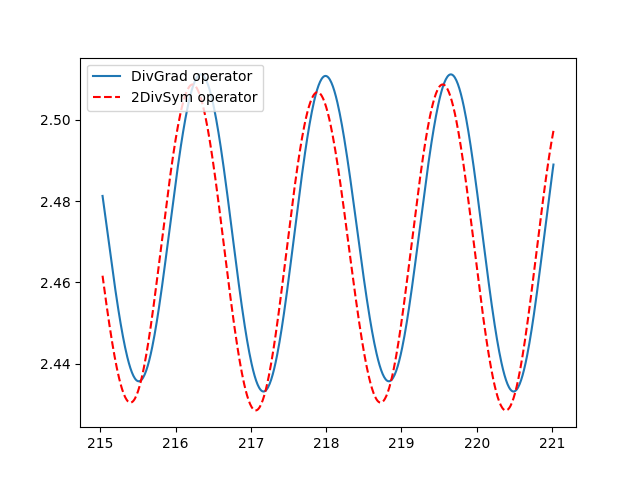
\includegraphics[width=0.5\linewidth]{PressureDifference.png}
	\caption{The pressure difference of both formulations}
	\label{Fig:Pressure}
\end{figure}
\begin{figure}
	\centering
	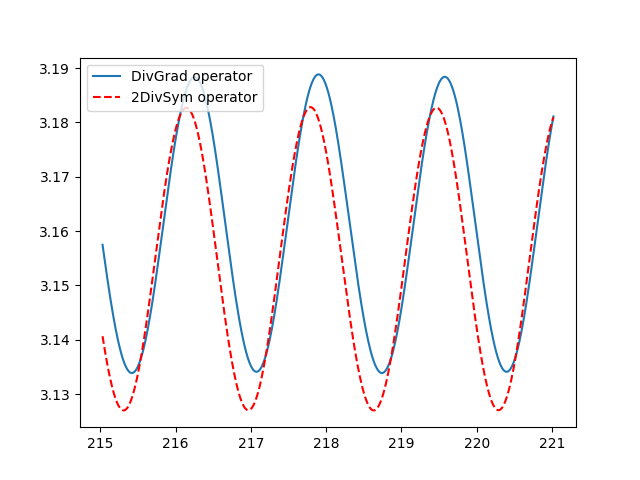
\includegraphics[width=0.5\linewidth]{DragCoefficient.png}
	\caption{The drag coefficient of both formulations}
	\label{Fig:Drag}
\end{figure}
\begin{figure}
	\centering
	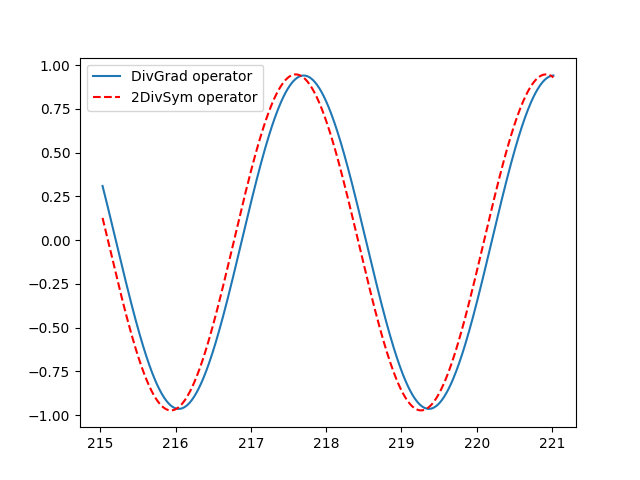
\includegraphics[width=0.5\linewidth]{LiftCoefficient.png}
	\caption{The lift coefficient of both formulations}
	\label{Fig:Lift}
\end{figure}
As you see, the results coincide in a pretty decent manner with those of the benchmark now. \textbf{According to the Remark 10.1 of the \textsc{Guermond} paper, one may enforce the \cref{Eqn:CylinderForce} if one also replaces the \textsc{Laplace} operator in the diffusion step by $\nabla \cdot \Sym (\nabla \otimes \bs{u})$. The thing is, that \textsc{Laplace} operator is applied always to the velocity field $\bs{u}$, independent of which projection scheme is used or if the divergence free velocity $\bs{v}$ was eliminated or not. Should not the \textsc{Laplace} operator be always replaced by the divergence of the symmetric operator?\\
I did another simulation where modified the weak form pertinent to the divergence of the velocity gradient. As seen in \crefrange{Fig:Pressure}{Fig:Lift}, the values (Labeled 2DivSym) are also inside the benchmark range. But the solution behave weird near the inflow boundary. I uploaded a video with the results of using the \textsc{Laplace} operator named "Laplace.ogv" and another one using the $\nabla \cdot \Sym (\nabla \otimes ())$ operator named "Transpose.ogv". In the  "Transpose.ogv" file you can see the mentioned weird behaviour. This might be due to the time step size, the spatial discretization, or the $\nabla \cdot \Sym (\nabla \otimes ())$ operator. But I wanted to discuss the last option before doing tests.}

\end{document}
